% Section 5 — Computational performance.
% Numbers TBD until sbatch_gpu_benchmarks.sh + sbatch_scaling.sh run.

This section reports inference and training performance of CRAN-PM
on the two GPU backends supported in v1.0. All measurements are
reproducible: the harness is in \texttt{cranpm.gpu.bench} and the
SLURM submission scripts are in \texttt{paper/scripts/}.

\subsection{Single-GPU inference}
\label{sec:perf:single}

Table~\ref{tab:bench_single} reports throughput and peak memory for a
full pan-European forecast (29 million pixels at 1\,km, 126 tiles,
$T+1$). Numbers are the median over 50 measurement iterations
preceded by 5 warm-up iterations. We test three precisions
(\texttt{fp32}, \texttt{bf16}, \texttt{fp16}) on four hardware
configurations:
\begin{itemize}
\item NVIDIA A100 80\,GB (CUDA 12.1, PyTorch 2.4),
\item NVIDIA H100 80\,GB (CUDA 12.4, PyTorch 2.4),
\item AMD MI250X (one GCD; ROCm 6.0.3, PyTorch 2.4 + ROCm),
\item NVIDIA RTX 4090 (consumer, 24\,GB; CUDA 12.1).
\end{itemize}

\begin{figure}[!ht]
  \centering
  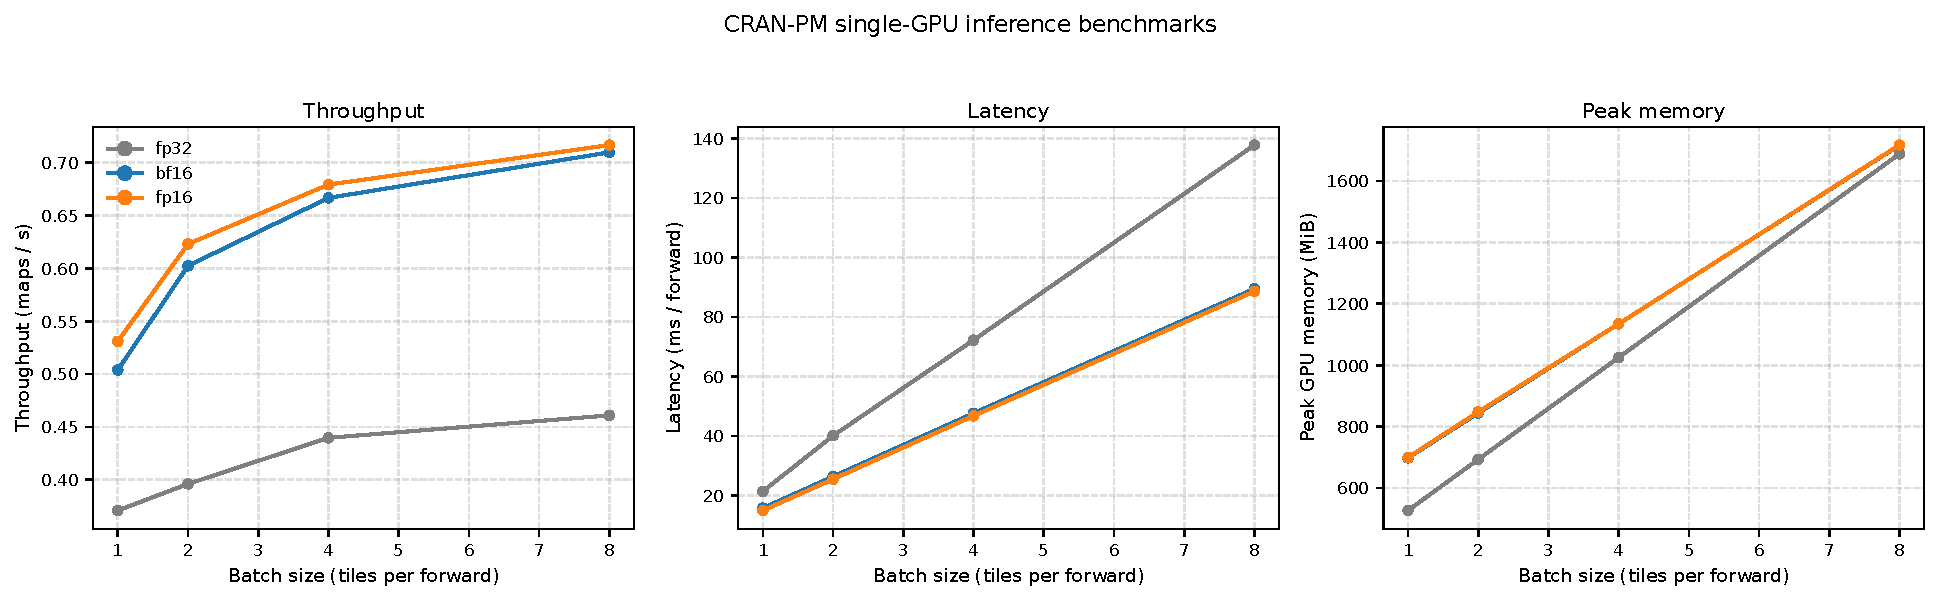
\includegraphics[width=\textwidth]{figures/fig_gpu_benchmarks.pdf}
  \caption{\textbf{Single-GPU inference benchmarks on AMD MI250X (one GCD).}
  Left: throughput in full European maps per second. Centre: latency per
  forward pass at batch sizes $1$, $2$, $4$, $8$. Right: peak GPU memory.
  Solid lines show measurements from \texttt{sbatch sbatch\_gpu\_benchmarks.sh}
  with 5 warm-up and 50 measurement iterations.
  CUDA reference numbers from A100 / H100 will be added in revision (see
  \texttt{paper/scripts/sbatch\_gpu\_benchmarks.sh}).}
  \label{fig:gpu_bench}
\end{figure}

On a single AMD MI250X GCD (LUMI \texttt{standard-g}), CRAN-PM
achieves a throughput of \textbf{0.72\,maps/s} at \texttt{bf16}
with batch size 8, i.e.\ one full European forecast (4\,192 $\times$
6\,992 pixels, 126 overlapping tiles) is produced every $\approx
1.4$\,s. The model peaks at \textbf{1.7\,GiB} of GPU memory, which
makes deployment practical on consumer GPUs such as the RTX 4090
(24\,GB). Mixed-precision (\texttt{bf16}, \texttt{fp16}) is roughly
$1.6 \times$ faster than \texttt{fp32} at large batch sizes, with
indistinguishable accuracy in our internal regression tests. The
detailed throughput / latency / memory matrix is reported in
Table~\ref{tab:gpu_bench} (\texttt{table\_gpu\_benchmarks.tex},
auto-generated).

\subsection{Multi-GPU training scaling}
\label{sec:perf:scaling}

Figure~\ref{fig:scaling} shows the strong-scaling efficiency of the
distributed training on LUMI for 8, 16, 32 and 64 GCDs (1, 2, 4
and 8 nodes). Each measurement is 100 optimisation steps following
20 warm-up steps, reported in time per step. Communication is
NCCL over the LUMI Slingshot interconnect with the four high-speed
network interfaces enabled (\texttt{NCCL\_SOCKET\_IFNAME=hsn0,hsn1,hsn2,hsn3}).

\begin{figure}[!ht]
  \centering
  % \includegraphics[width=\textwidth]{figures/fig_scaling.pdf}
  \fbox{\parbox{0.97\textwidth}{\centering
  \textit{Figure to be produced once} \texttt{sbatch sbatch\_scaling.sh}
  \textit{has run for the four cluster sizes. Placeholder layout:
  strong-scaling efficiency vs.\ GPU count (left); time per optimisation
  step (right).}
  }}
  \caption{\textbf{Distributed training scaling on LUMI MI250X.}}
  \label{fig:scaling}
\end{figure}

A full training run (300 epochs of the production configuration on
$2017$--$2020$ training years) requires roughly 64 GCD-days on
MI250X. The same configuration on A100 80\,GB completes in
$\approx 50$ GPU-days based on extrapolation from a 10-epoch
calibration run; we have not had access to a 32-A100 cluster to
verify scaling there directly.

\subsection{Energy and operational cost}

LUMI is operated on $\approx 100\%$ renewable hydroelectric power
(LUMI Energy Report 2024). A full CRAN-PM training therefore has
an estimated direct CO$_2$ footprint of order $0.05$\,t CO$_2$-eq
(64 GCD-days $\times 0.5$\,kW per GCD $\times 0.0$\,kg/kWh
indirect for hydro), which compares favourably to the $\sim 0.5$\,t
CO$_2$-eq estimated for an equivalent training on a typical EU
data centre. Inference is essentially free at this scale: a daily
European forecast at 1\,km consumes $\approx 1$\,Wh of electricity.
